\documentclass[a4paper,10pt]{article}

\usepackage{lipsum}
\usepackage[english]{babel}
\usepackage[margin=15mm]{geometry}
\usepackage{amsmath}
\usepackage{amssymb}
\usepackage{graphicx}
\usepackage{subfigure}

\title{Multi-Agent Systems Summative Assignment}
\date{\today}
\author{James King}

\begin{document}
\maketitle

\section{Application Specification}
\subsection{Overview}
\paragraph{World}
The task is a simple turn-based game within a tile based world, where two or more teams of bots compete for survival. Each team starts with one or more \emph{home} tiles, upon which a bot belonging to that team begins. Every remaining tile in the world may be a solid \emph{wall}, a \emph{resource} item, a \emph{bot}, or \emph{empty}. The world is a two dimensional grid of fixed dimensions, and has the topology of the surface of a torus (travelling off one side of the grid will bring you to the opposite side). The world is initially unknown to players of the game, but at the start of each turn every player is given the state of previously undiscovered tiles that are within a certain fixed \emph{vision radius} of any agent on their team. The locations of resources, along with the positions, team affiliation and direction of agents within the vision radius is also given before each turn.

\begin{figure}[ht]
  \centering
  \mbox{
    \subfigure
      [The blue bot moves to eliminate the pink bot.]
      {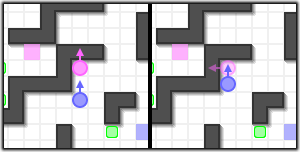
\includegraphics[width=0.45\linewidth]{kill}}
    \quad
    \subfigure
      [Mutual elimination when two bots occupy the same tile.]
      {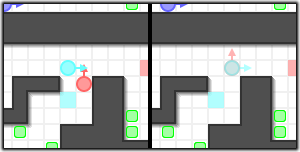
\includegraphics[width=0.45\linewidth]{mutual}}
  }
  \caption{Demonstrations of the two rules for bot elimination.}
  \vspace{-5mm}
\end{figure}

\paragraph{Bots}
Bots have a \emph{direction} property, which may be any one of the cardinal directions (\emph{north}, \emph{east}, \emph{south}, or \emph{west}). Each turn, each team decides a single action to perform with each bot belonging to them. This action may be to rotate the bot \emph{left} or \emph{right} (so a bot that was facing east which turns left will now face north), to \emph{move} one tile in the direction it is currently facing (unless a wall is in the destination tile, in which case it does not move), or to \emph{pass} and do nothing. After each team decides on a set of moves, all the bots commit to their assigned instruction simultaneously. If any two or more bots occupy the same tile they are removed from the world before the next turn. Also, a bot is removed if it is neighbouring another bot of a different team that is facing it.


\paragraph{Resources}
Resources are items that appear at regular intervals in the world on randomly selected empty tiles. These are initially stationary, but if a bot appears on a neighbouring tile and faces the resource, the bot begins to \emph{carry} the resource which will attempt to remain one tile in front of the carrying bot. If the carrying bot moves forward, the resource is \emph{pushed} in the direction the bot moved by one tile. If the bot turns, the resource will move to whichever tile the bot is now facing. However, if the destination tile for the resource when either pushed or turned isn't vacant, the resource is removed from the world. Finally, if the resource is moved to a home tile, a new bot belonging to the home tile's corresponding team is created in its place.

\begin{figure}[ht]
  \centering
  \mbox{
    \subfigure
      [Moving a resource (green) onto a home tile spawns a new bot and consumes the resource.]
      {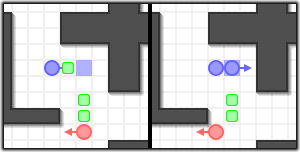
\includegraphics[width=0.45\linewidth]{capture}}
    \quad
    \subfigure
      [Pushing a resource into a wall, bot, or another resource will remove it.]
      {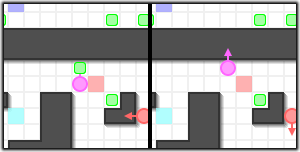
\includegraphics[width=0.45\linewidth]{destroy}}
  }
  \caption{Demonstrations of resource consumption and destruction.}
  \vspace{-5mm}
\end{figure}

\paragraph{Solution Requirements and Interfaces}
Each team will have a single program that controls all of the bots on their team. Each program is initially given the dimensions of the world, number of teams, vision radius and allowed time per turn over standard input, and then at the start of each turn they provided with given the tile, resource and bot information as previously specified. Each team's program is then expected to produce an action for each bot over standard output, and upon the arrival of all instructions the game moves to the next turn. If any team's program fails to produce its set of actions before the allotted time has elapsed, all bots belonging to that team are eliminated and its program terminated. Each controller program may be implemented in any language that supports standard input and output operations.

\paragraph{End Conditions and Goals}
The game lasts until either a predetermined turn limit is reached, or only bots belonging to one team remain. When the game ends, whichever team has the most remaining bots is declared the winner. The aim of the game is therefore to try and eliminate as many bots belonging to opposing teams as possible, while attempting to transport resources back to a home tile owned by your team and preventing other teams from doing so.

\subsection{Task Environment Identification}
A useful initial step when designing any kind of system involving agents is to classify the environment in terms of how it is perceived by and reacts to agents, and to recognise exactly which behaviours should be encouraged in agents. These properties of the task are usually known as the \emph{performance measure}, \emph{environment properties}, \emph{actuators} and \emph{sensors}, or the \emph{PEAS}, as discussed by Norvig and Russel in Artificial Intelligence: A Modern Approach\cite{norvig10}.

\paragraph{Performance Measure}
As this is a cooperative system (at least with respect to the bots belonging to one team), where the cooperating bots reside in the same program, performance may be measured for the team as a whole and not for each bot independently. Each team is attempting to maximise their number of active bots, while reducing the number of bots in opposing teams. This can be expressed as a ratio of active bots belonging to the measured team against the total number of active bots. However, this would suggest that a scenario where 5 bots are split between three teams $(A, B, C)$ using the distribution $(2, 2, 1)$ is equivalent to the distribution $(2, 3, 0)$ for team $A$. This should not be the case, as in the first scenario team $A$ is tied in first place with team $B$, but in the second scenario team $A$ is in second place and so should have a lower performance measure. One possible revised performance measure expression that resolves this is the following:

\begin{figure}[ht]
  \centering
  \begin{minipage}{0.8\textwidth}
    $$
      \text{performance}\left(\text{team}\right) = \frac
        {\left|\text{bots} \cap \text{team}\right|^2}
        {\sum_{t \in \text{teams}} \left|\text{bots} \cap \text{t}\right|^2}
    $$
    \caption{A performance measure expression that takes into account the number of bots belonging to opposing teams.}
  \end{minipage}
\end{figure}

\noindent
This performance measure can differentiate between distributions of agents between teams where the original expression could not, so eliminating bots from a larger (and therefore more threatening) opposing team would provide more utility than doing so from a small one. Maximizing this score will increase the probability of winning the game, and in fact as soon as the performance score for a given team reaches $1.0$ that team must win, because all opposing agents have been eliminated.

\paragraph{Environment Properties}
Using the definitions provided by Russel and Norvig\cite{norvig10}, the environment is \emph{partially observable} due to how only the contents of tiles near to bots are revealed to the team each bot belongs to. Naturally, it is a \emph{multi-agent} system that is both \emph{cooperative} (between agents belonging to the same team) and \emph{competitive} (between agents belonging to distinct teams). The environment is slightly \emph{stochastic} due to the random distribution of resources over time, and \emph{uncertain} because of its stochastic nature, the presence of other agents, and because it is partially observable. Turns are \emph{sequential} rather than episodic because each choice may affect every following one. Environment state and the intervals between percepts are \emph{discrete} since the world is aligned to a grid and time is divided into turns, and the environment is mostly static except for the maximum turn time limit which renders it \emph{semidynamic}. Finally, the outcomes of actions are \emph{known} because they always produce an expected result for some localised aspect of the environment.

\paragraph{Actuators and Sensors}
Each team can interact with the environment by selecting an action from the set of allowed actions for each of their bots. Percepts include several elements; first is a subset of previously undiscovered tiles revealing their state (either empty, a wall, or a home tile for a specified team), then the locations of visible bots along with their team and the direction they are facing, and finally the locations of visible resources.

\section{Scenarios}
A solution for this task should be able to act in the ways suggested in the following situations. Of course, two or more of the opportunities detailed here can crop up simultaneously, so the solution should evaluate which is expected to be more beneficial to pursue. Many more scenarios may emerge that do not fit into any of these templates, so the solution should account for unexpected events also. In the following scenarios, `bot' will refer to bots controlled by the solution program, and `opponents' will refer to the rest of the bots.

\newcommand{\scenario}[4]{
  \subsection{#1}
  \paragraph{Description}
  #2

  \vspace{-3mm}
  \paragraph{Start Condition}
  #3

  \vspace{2mm}
  \begin{center}
  \begin{tabular}{r l l l}
    ~ & \textbf{Steps} & \textbf{Functionality} & \textbf{Data} \\
    #4
  \end{tabular}
  \end{center}
}

\scenario{Capture Resource}{
  A resource is identified as being easy to capture, and is escorted to a home tile by a bot.
}{
  Resource seen near bot and risk is estimated to be below some threshold.
}{
  1. & Resource seen near bot & World Observation & Resources \\
  2. & Evaluated to be capturable without risk & Risk Evaluation & Opponents, World Tiles \\
  3. & Bot navigates to resource & Path Finding & World Tiles \\
  4. & Bot navigates back to a home tile & Path Finding & World Tiles \\
  5. & Resource is not pushed into walls / bots & World Observation & World Tiles \\
}

\scenario{Hinder Opponent Resource Capture}{
  A resource is identified as being easier for an opposing team to capture, and is removed by being pushed into a wall to hinder their efforts.
}{
  Resource seen near bot and risk is estimated to be below some threshold for some opposing team.
}{
  1. & Resource seen near bot & World Observation & Resources \\
  2. & Evaluated to be easier for an opponent to capture & Risk Evaluation & Opponents, World Tiles \\
  3. & Bot navigates to resource & Path Finding & World Tiles \\
  4. & Nearby wall tile found & World Observation & World Tiles \\
  5. & Bot pushes resource into wall & Path Finding & World Tiles \\
}

\scenario{Eliminate Opponent}{
  A vulnerable opponent is forced into an inescapable position, and is eliminated when the potential risk is deemed low enough.
}{
  A single opponent shares a locality with several bots on this team.
}{
  1. & Several bots encounter single opponent & World Observation & Opponents \\
  2. & Bots approach opponent when safe & Risk Evaluation & Opponents \\
  3. & Opponent becomes blocked & Opponent Consideration & Opponents, World Tiles \\
  4. & Bots await opportunity to safely strike & Risk Evaluation & Opponents
}

\scenario{Defend Trapped Bot}{
  A vulnerable bot is surrounded by opponents, but other bots arrive to assist.
}{
  A single bot shares a locality with several opponents, with other bots nearby to assist.
}{
  1. & Bot is blocked by opponents & Opponent Consideration & Opponents, World Tiles \\
  2. & Another bot approaches a blocking opponent & Path Finding & Opponents, World Tiles \\
  3. & Bot waits until opponent is vulnerable & Risk Evaluation & Opponents \\
  4. & Approaching bot strikes opponent & World Observation & Opponents \\
}

\newpage
\section{Agent Role Division}
\vspace{-5mm}
\begin{figure}[ht]
  \centering
  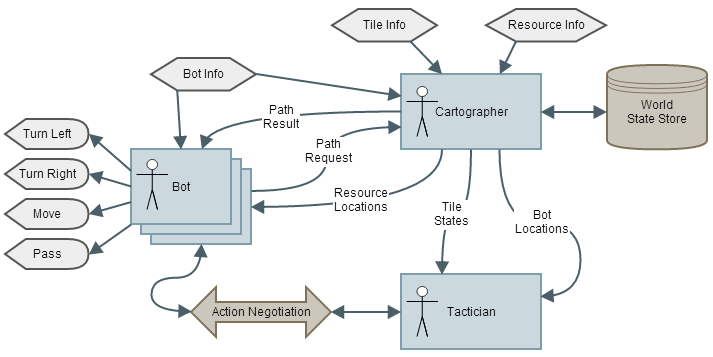
\includegraphics[width=0.8\linewidth]{interaction}
  \caption{Diagram showing the main interactions between the three proposed agent classes.}
  \vspace{-5mm}
\end{figure}
\vspace{5mm}

\paragraph{Bot Agent}
The most obvious recognisable agent class in the system is the \emph{Bot} agent. Each bot belonging to the team would have a separate Bot agent assigned to it, which would control self preservation of that bot and the following of any plans assigned to that bot by other agents. The Bot agent would delegate planning and most deliberation to other agents in the system, and mostly follow their instructions with some reactive mechanisms for avoiding danger. Because of this, a subsumptive architecture\cite{brooks90} would be a good fit for the overall design of the agent.

\paragraph{Cartographer Agent}
A solution for this task should attempt to record the structure of the environment to be recalled when previously visible aspects of it are hidden. It would be wasteful for each Bot agent to hold a separate representation of the world, and so a static structure external to them would be best. While maintaining this structure is reasonably simple, an effort should be made by the solution to attempt to explore regions of the environment that were previously undiscovered, or to revisit areas to keep an eye on enemy activity. For that, a \emph{Cartographer} agent could attempt to decide which areas are most worth visiting, and could distribute exploration tasks among Bot agents. The Cartographer would also be in charge of maintaining the world representation, and so use relevant percepts to update the structure. It would also service requests by other agents as to the state of some region of the environment. Finally, the agent could plan which resources are worth capturing or destroying, and assign agents to do either while avoiding assigning multiple agents to perform the same task. The agent would have several competing goals to achieve at any time, and should decide which to commit to. It is for this reason a Belief-Desires-Intentions architecture may be most fitting.

\paragraph{Tactician Agent}
The remaining functionality not captured by the first two agent classes relate to interaction with enemy bots, and so a \emph{Tactician} agent may be constructed to deal with hindering, avoiding or eliminating opposing bots. While the Cartographer will retain the last known locations of enemy bots, the Tactician will query that information to be used when deliberating actions. 

\section{Bot Agent (Subsumptive)}
\begin{figure}[ht]
  \centering
  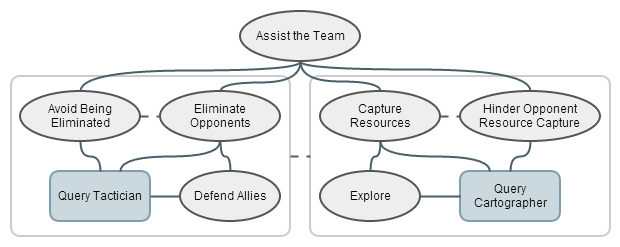
\includegraphics[width=0.7\linewidth]{bot}
  \begin{minipage}[t]{0.8\textwidth}
    \caption{A breakdown of the Bot agent's main functions into sub-functions, with possible conflicts of interest represented by dashed lines.}
  \end{minipage}
\end{figure}

\section{Cartographer Agent (BDI)}
\begin{figure}[ht]
  \centering
  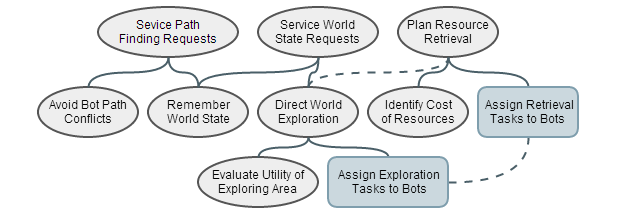
\includegraphics[width=0.7\linewidth]{cartographer}
  \begin{minipage}[t]{0.8\textwidth}
    \caption{A breakdown of the Cartographer agent's main functions into sub-functions, with possible conflicts of interest represented by dashed lines.}
  \end{minipage}
\end{figure}

\section{Tactician Agent (Hybrid)}

\begin{thebibliography}{9}
  \bibitem{norvig10}
    Stuart Russell and Peter Norvig,
    \emph{Artificial Intelligence: A Modern Approach}. \newline
    Pearson Education Inc.,
    3rd Edition,
    2010.

  \bibitem{brooks90}
    Rodney Brooks,
    \emph{Elephants Don't Play Chess}. \newline
    Robotics and Autonomous Systems,
    Volume 6,
    1990.

  \bibitem{rao}
    Anand Rao and Michael Georgeff,
    \emph{BDI Agents: From Theory to Practice}. \newline
    Proceedings of the First International Conference on Multi-Agent Systems,
    1995.
\end{thebibliography}

\end{document}
